\chapter{Công nghệ phát triển}

\section{Công nghệ Phát triển Ứng dụng Di động Đa nền tảng}

Việc lựa chọn nền tảng phát triển là yếu tố then chốt quyết định tính phổ dụng và hiệu năng của Ứng dụng trải nghiệm (Player). Khóa luận đã chọn sử dụng Flutter và ngôn ngữ Dart để phát triển ứng dụng di động.

\subsection{Giới thiệu về Flutter và Ngôn ngữ Dart}

Flutter là một bộ công cụ phát triển giao diện người dùng được Google phát triển, cho phép xây dựng ứng dụng di động, web, và desktop từ một codebase duy nhất. Ngôn ngữ lập trình chính được sử dụng là Dart.

Việc lựa chọn Flutter mang lại những lợi thế chiến lược quan trọng. Thứ nhất, khả năng \textbf{đa nền tảng} cho phép triển khai ứng dụng đồng thời trên cả Android và iOS mà không cần phát triển lại, giúp tiết kiệm thời gian và chi phí. Thứ hai, Flutter được biết đến với \textbf{hiệu năng cao} do sử dụng công cụ kết xuất đồ họa riêng, giúp giao diện người dùng chạy mượt mà, rất quan trọng đối với một ứng dụng bản đồ cần cập nhật vị trí và hình ảnh liên tục.

\subsection{Sử dụng Google Maps Platform}

Để thực hiện chức năng hiển thị bản đồ và định vị, hệ thống TMAP tích hợp sâu với Google Maps Platform. Thư viện này cung cấp các API cần thiết để: \textbf{hiển thị bản đồ} chi tiết trên ứng dụng di động và trình biên soạn Web, \textbf{định vị chính xác} vị trí của người dùng, và \textbf{quản lý các điểm đánh dấu} (Markers) của các điểm tham quan trên Map trải nghiệm. Việc sử dụng Google Maps đảm bảo dữ liệu bản đồ luôn được cập nhật và có độ tin cậy cao về mặt địa lý.

\section{Công nghệ Phát triển Web và Backend}

Hệ thống TMAP yêu cầu một nền tảng Backend mạnh mẽ và linh hoạt để quản lý cơ sở dữ liệu và xử lý các yêu cầu từ cả Trình biên soạn và Ứng dụng trải nghiệm.

\subsection{Sử dụng Framework Laravel và Ngôn ngữ PHP}

Laravel là một framework PHP mã nguồn mở, được sử dụng để xây dựng Trình biên soạn Web và hệ thống API Backend cho TMAP. Laravel cung cấp các tính năng bảo mật, quản lý phiên và quản lý cơ sở dữ liệu hiệu quả, tạo điều kiện thuận lợi cho việc phát triển nhanh và ổn định. PHP là ngôn ngữ backend được lựa chọn vì tính phổ biến, cộng đồng lớn và khả năng xử lý các tác vụ phức tạp liên quan đến quản lý dữ liệu đa phương tiện.

\subsection{Kiến trúc Microservices và RESTful API}

Nền tảng Trealet hoạt động theo kiến trúc \textbf{Microservices}, trong đó TMAP được coi là một Service độc lập chịu trách nhiệm quản lý tất cả các dữ liệu liên quan đến bản đồ và tuyến trải nghiệm. Các Service này giao tiếp với nhau và với các ứng dụng Client (Editor và Player) thông qua \textbf{RESTful API}. RESTful API đảm bảo tính đồng bộ, bảo mật và khả năng mở rộng của hệ thống. Dữ liệu được trao đổi chủ yếu dưới dạng JSON, cho phép Flutter Player dễ dàng tiếp nhận và xử lý.

\section{Kiến trúc Tổng quan của Nền tảng Trealet và Vị trí của TMAP}

Kiến trúc tổng thể của Trealet là một hệ thống phân tán, được thiết kế để xử lý đa dạng các loại nội dung và trải nghiệm văn hóa. TMAP không phải là một ứng dụng độc lập mà là một \textbf{hệ thống con (Microservice)} cốt lõi trong Trealet, chuyên trách về việc tạo lập và phân phối các trải nghiệm dựa trên vị trí địa lý.

Luồng dữ liệu trong kiến trúc Trealet được thiết lập với Trình biên soạn Web gửi dữ liệu Map mới tới API của TMAP Service. Dữ liệu được lưu trữ trong cơ sở dữ liệu chuyên biệt của TMAP. Ứng dụng trải nghiệm di động (Player) truy vấn các Map có sẵn thông qua các RESTful API của TMAP Service. Toàn bộ quy trình này đảm bảo tính nhất quán của dữ liệu và khả năng tích hợp TMAP một cách liền mạch vào các thành phần khác của nền tảng Trealet, ví dụ như hệ thống xác thực người dùng hoặc hệ thống lưu trữ đa phương tiện.

Kiến trúc tổng thể của nền tảng Trealet và TMAP được biểu diễn chi tiết trong \figurename~\ref{fig:KientrucTrealet} và \figurename~\ref{fig:KienTrucTMAP}.

\begin{figure}[h]
    \centering
    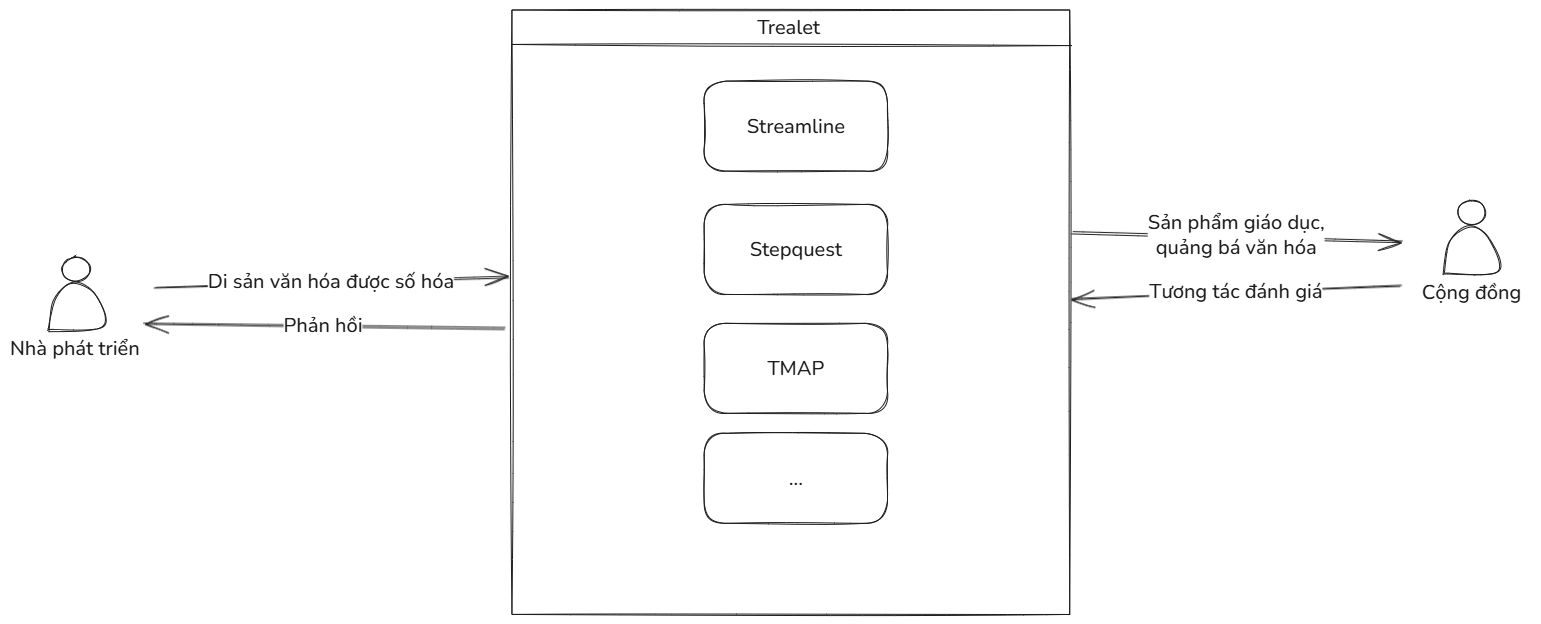
\includegraphics[width=0.9\textwidth]{Hinh_Kien_Truc_Trealet.png} % Thay bằng tên file hình ảnh thực tế
    \caption{Kiến trúc tổng thể của nền tảng Trealet}
    \label{fig:KientrucTrealet}
\end{figure}

\begin{figure}[h]
    \centering
    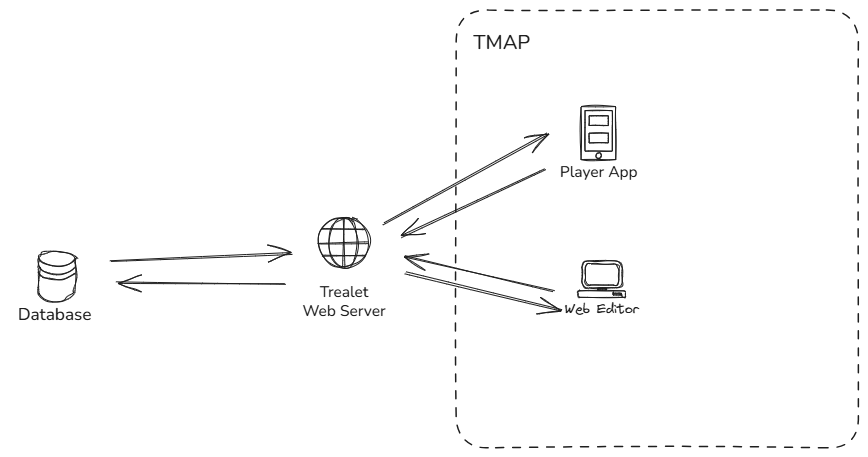
\includegraphics[width=0.8\textwidth]{tmap_design.png} % Thay bằng tên file hình ảnh thực tế
    \caption{Kiến trúc tổng quan của TMAP}
    \label{fig:KienTrucTMAP}
\end{figure}